\chapter{Logical Reasoning with Diagrams}
\label{sec:p12-rationality-13-1}

A diagram can be part of a proof rather than merely an illustration of
one. Its logical standing depends on what its marks mean and which
transformations preserve the represented information. Jamnik's 2021
treatment addresses this question from computational, algorithmic and
software-implementation perspectives. It compares formal diagram
languages and three implemented reasoning systems, while distinguishing
the search for a correct answer from the search for an explanation a
person can understand \cite[pp.~715--723]{Jamnik2021LogicalDiagrams}.
Here \emph{implementational} concerns software executing a reasoning
task, not a claim about the hardware embodying human rationality.

This is not the mental-rotation task in
\cref{sec:p19-mental-rotation}. Bringing two shapes into congruence and
measuring response time does not establish a diagrammatic inference
calculus. Nor is a diagram automatically a model of someone's internal
representation. The questions here are how an external representation
expresses premises, what follows from them, and how a machine can check
the inference.

\section{Representation, explanation and the coloring invariant}

Jamnik presents a tension between mathematicians' longstanding use of
figures and a conception of proof requiring explicit axioms and checked
steps independent of a persuasive drawing. Her historical discussion
contrasts Euler, Venn and Peirce's diagrammatic projects with the rise of
symbolic formalization, and points to deceptive mathematical pictures.
This is a bounded history of the problem, not a proof that all earlier
diagrams lacked logical rules. Peirce's 1933 collected papers are not a
date for the first invention of every diagram in that collection.
Hilbert's 1894 lecture and its 2004 published edition likewise have
different dates. Its selected cautionary example is Cauchy's visual
argument for Euler's polyhedron theorem as analyzed by Lakatos; the
longstanding acceptance of an argument is not a soundness proof.
The source's Newton note warns that a geometric argument
can later be presented through a symbolic calculus; symbolic versus
diagrammatic is not a simple historical or philosophical dichotomy
\cite[pp.~715,722, notes~1--2]{Jamnik2021LogicalDiagrams}.

The positive proposal is that a formal diagram can carry the reason a
solution works. Human-oriented systems seek accessible explanations;
machine-oriented systems may instead optimize deciding theoremhood,
proof-search speed or the number of problems solved. These are different
design objectives, not mutually exclusive kinds of correctness. A
rigorous diagram language removes the objection that figures cannot
have syntax, semantics or sound proof rules; it does not remove all
questions about their clarity or suitability. Jamnik contrasts this
human-like reasoning motivation with mainstream statistical-learning
motivations in AI; she does not identify one historical research emphasis
with every possible AI system or make it a current-software guarantee.

\begin{hbexample}{def:p12-r131-checkerboard}{The mutilated checkerboard}
Take an \(8\)-by-\(8\) board of unit cells. Delete the upper-left and
lower-right cells. A domino covers exactly two edge-adjacent cells,
without overlaps or gaps. Figure~\ref{fig:p12-r131-checkerboard}
re-presents the source's uncolored and colored boards. Searching through
tilings obscures a simple invariant: every permitted domino occupies
one cell of each color, but the two removed cells have the same color.
The representation changes what is easy to detect, not the tiling rules
or the object being investigated.
\end{hbexample}

\begin{figure}[htbp]
\centering
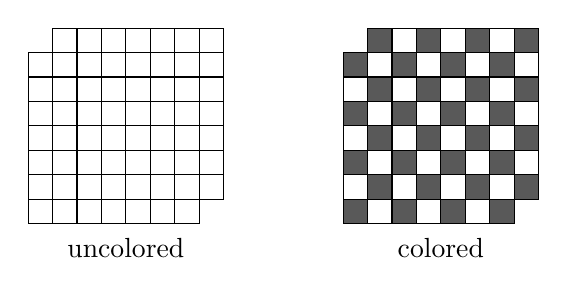
\begin{tikzpicture}[x=.31cm,y=.31cm]
\foreach \i in {0,...,7}{\foreach \j in {0,...,7}{
  \pgfmathtruncatemacro{\omitcell}{(\i==0 && \j==7)||(\i==7 && \j==0)}
  \ifnum\omitcell=0 \draw (\i,\j) rectangle +(1,1);\fi}}
\node at (4,-1) {uncolored};
\begin{scope}[xshift=4cm]
\foreach \i in {0,...,7}{\foreach \j in {0,...,7}{
  \pgfmathtruncatemacro{\omitcell}{(\i==0 && \j==7)||(\i==7 && \j==0)}
  \pgfmathtruncatemacro{\paritycell}{mod(\i+\j,2)}
  \ifnum\omitcell=0
    \ifnum\paritycell=0 \fill[black!65] (\i,\j) rectangle +(1,1);\fi
    \draw (\i,\j) rectangle +(1,1);
  \fi}}
\node at (4,-1) {colored};
\end{scope}
\end{tikzpicture}
\caption{Native vector reconstruction of the two checkerboard
representations in Jamnik's figures~13.1.1--2. Coloring exposes a
necessary invariant of an exact domino tiling.}
\label{fig:p12-r131-checkerboard}
\end{figure}

\begin{hbtheorem}{thm:p12-r131-checkerboard}{proved=annex:p12.r131.checkerboard}{The deleted-corner board is not domino-tileable}
Under exactly the edge-adjacent, disjoint, exact-cover assumptions of
\cref{def:p12-r131-checkerboard}, the board has no domino tiling.
\end{hbtheorem}

The conclusion fails to transfer to a tile allowed to occupy two
nonadjacent cells or to overlap another tile. Conversely, equal color
counts are only necessary: they do not suffice for arbitrary mutilated
boards. For example, the retained cells \((1,1)\) and \((4,3)\) have
opposite parity but are not adjacent, so cannot form a single domino.
The invariant excludes the stated board without proving a general
tiling algorithm.

The example motivates representation selection. Jamnik draws on P\'olya,
Amarel, Simon and Anderson to relate representation to the processes
operating on it, and on Larkin and Simon to explain why a useful diagram
can reduce search. \Cref{def:p12-heuristic-problem} already requires
preserving data, conditions and the requested output when transforming
a problem. Discovering the coloring is a heuristic act; once it is
chosen, the impossibility claim has a deductive justification. A proof
of that justification is not a psychological measurement of how often
people discover it.

\section{Free rides and the declared meaning of a region}

\begin{hbdefinition}{def:p12-r131-region-reading}{Set interpretation and incidental geometry}
In the following set-diagram examples, contour labels name subsets of
a common universe \(U\). Containment expresses inclusion; exclusion of
a membership zone expresses that the represented set is empty. A region
label is not a name for an individual. No existential import follows
merely from the area enclosed by a curve. Curve radius, left/right
position and physical area have no set-cardinality meaning here.
An Euler diagram can omit zones; a full Venn diagram draws every Boolean
membership zone and can use shading to state emptiness instead.
\end{hbdefinition}

\begin{hbexample}{def:p12-r131-free-ride}{An Euler free ride}
The premises \(P\cap Q=\varnothing\) and \(R\subseteq P\) can
be expressed by placing the \(R\)-contour within \(P\), away from
\(Q\). The resulting picture also displays \(R\cap Q=\varnothing\).
Shimojima's \emph{free ride}, as used by Jamnik, is information forced
by representing other information, rather than information added as a
new premise \cite[p.~717, fig.~13.1.3]{Jamnik2021LogicalDiagrams}.
\end{hbexample}

\begin{figure}[htbp]
\centering
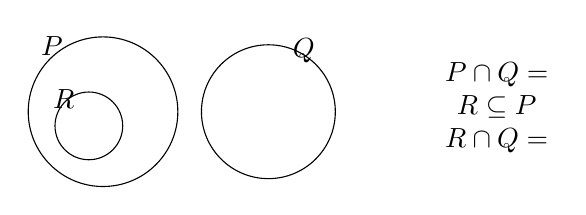
\begin{tikzpicture}[x=1cm,y=1cm]
\draw (0,0) circle (.95); \node at (-.65,.83) {$P$};
\draw (-.18,-.18) circle (.43); \node at (-.5,.16) {$R$};
\draw (2.1,0) circle (.85); \node at (2.55,.78) {$Q$};
\node[align=center] at (5,.05) {$P\cap Q=\varnothing$\\$R\subseteq P$\\$R\cap Q=\varnothing$};
\end{tikzpicture}
\caption{Euler representation of the source's free ride. Inclusion and
empty intersection have declared meanings; the drawn areas do not
assert that any of the sets is nonempty.}
\label{fig:p12-r131-euler}
\end{figure}

\begin{hbtheorem}{thm:p12-r131-free-ride}{proved=annex:p12.r131.free-ride}{Validity of the displayed free ride}
For subsets \(P,Q,R\subseteq U\),
\(P\cap Q=\varnothing\) and \(R\subseteq P\) imply
\(R\cap Q=\varnothing\). The premises do not imply that \(R\)
is nonempty or that \(R=P\).
\end{hbtheorem}

A reader must check the interpretation before taking a visual relation
as a consequence. Drawing disjoint contours for an unspecified relation
can accidentally assert more than the premises. Choosing one possible
model and inspecting its extra relations is not the same as representing
all allowed models. The free ride above is legitimate because the
conclusion holds in \emph{every} interpretation of its premises.

\section{Venn, Euler and spider languages}

Jamnik attributes formal syntax, semantics and sound/complete inference
systems for Venn-I and Venn-II to Shin, and an Euler treatment to Hammer.
These are named systems with particular expressive resources, not
one generic calculus of pictures. Venn shading means emptiness; an
\(x\)-mark supplies an existential witness. A linked sequence of
\(x\)-marks places \emph{one} witness in a disjunction of regions,
not one witness in every marked region. Venn-II additionally links
\emph{whole diagrams} to express alternative assertions
\cite[pp.~717--718]{Jamnik2021LogicalDiagrams}.

Peirce's linked \(x\)- and \(o\)-marks indicated nonemptiness and
emptiness rather than using Venn's empty-zone shading; Jamnik notes
that such links can sacrifice some of the immediate spatial readability.

In the source's Venn-I example the Euler premises are supplemented by
\(Q\setminus(P\cup R)\ne\varnothing\) and
\(P\setminus Q\ne\varnothing\). The second witness's linked
positions leave its membership in \(R\) undecided. The Venn-II
example instead states
\[
 \bigl(P\subseteq Q\ \land\ Q\setminus P\ne\varnothing\bigr)
 \ \lor\ \bigl(R\setminus P\ne\varnothing\bigr).
\]
It does not assert both disjuncts. Thus Venn-I's limited disjunction of
witness locations must not be confused with Venn-II's disjunction of
whole diagram assertions. The former resource does not by itself give
arbitrary Boolean combinations of unitary diagrams.

\begin{figure}[htbp]
\centering
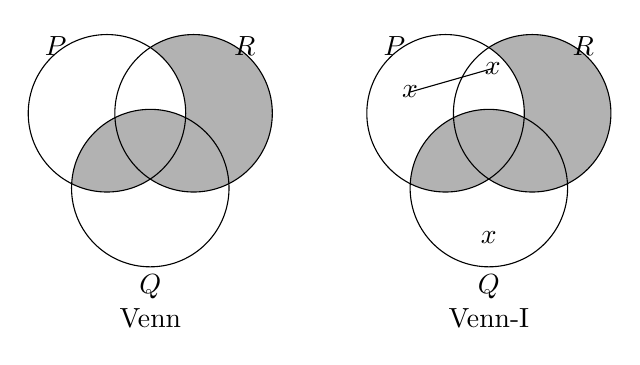
\begin{tikzpicture}[x=1cm,y=1cm]
\foreach \offset in {0,4.3}{
\begin{scope}[xshift=\offset cm]
\fill[black!30] (.55,.35) circle (1);
\begin{scope}\clip (-.55,.35) circle (1);
  \fill[white] (.55,.35) circle (1);\end{scope}
\begin{scope}\clip (-.55,.35) circle (1);
  \fill[black!30] (0,-.6) circle (1);\end{scope}
\draw (-.55,.35) circle (1); \draw (.55,.35) circle (1);
\draw (0,-.6) circle (1);
\node at (-1.2,1.2) {$P$}; \node at (1.2,1.2) {$R$};
\node at (0,-1.85) {$Q$};
\end{scope}}
\node at (0,-2.25) {Venn}; \node at (4.3,-2.25) {Venn-I};
\begin{scope}[xshift=4.3cm]
\draw (-1,.62)--(.05,.92);
\node at (-1,.62) {$x$}; \node at (.05,.92) {$x$};
\node at (0,-1.23) {$x$};
\end{scope}
\end{tikzpicture}
\caption{Full-zone Venn rendering of the free-ride premises (left),
and the source's Venn-I extra witnesses (right). Gray is empty.
The connected upper marks are alternatives for one witness in
\(P\setminus Q\); the lower mark gives a witness in
\(Q\setminus(P\cup R)\).}
\label{fig:p12-r131-venn}
\end{figure}

\begin{figure}[htbp]
\centering
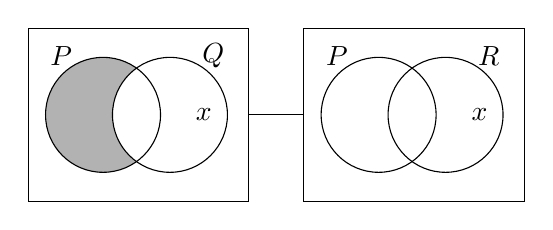
\begin{tikzpicture}[x=1cm,y=1cm]
\draw (-1.4,-1.1) rectangle (1.4,1.1);
\begin{scope}\clip (-.45,0) circle (.73);
 \fill[black!30] (-1.4,-1.1) rectangle (1.4,1.1);\end{scope}
\begin{scope}\clip (-.45,0) circle (.73);
 \fill[white] (.4,0) circle (.73);\end{scope}
\draw (-.45,0) circle (.73); \draw (.4,0) circle (.73);
\node at (-.98,.75) {$P$}; \node at (.95,.75) {$Q$};
\node at (.83,0) {$x$};
\draw (1.4,0)--(2.1,0);
\begin{scope}[xshift=3.5cm]
\draw (-1.4,-1.1) rectangle (1.4,1.1);
\draw (-.45,0) circle (.73); \draw (.4,0) circle (.73);
\node at (-.98,.75) {$P$}; \node at (.95,.75) {$R$};
\node at (.83,0) {$x$};
\end{scope}
\end{tikzpicture}
\caption{The two whole-diagram alternatives of the source's Venn-II
example. Their connecting line denotes disjunction, not conjunction;
it has a different syntactic role from a linked witness's line.}
\label{fig:p12-r131-venn-ii}
\end{figure}

\begin{hbdefinition}{def:p12-r131-spider-syntax}{Speedith's typed unitary spider syntax}
For the selected Speedith presentation a unitary diagram is
\(d=(L,Z,\mathrm{ShZ},S,\eta)\). Here \(L\) is a finite set of
contour labels; a zone \(z=(\mathrm{in},\mathrm{out})\) partitions
\(L\) into disjoint inside/outside labels. \(Z\) is the nonempty
set of present zones, \(\mathrm{ShZ}\subseteq Z\) the shaded zones,
and \(S\) the finite set of spiders. Each habitat
\(\eta(s)\) is a nonempty subset of \(Z\). In a drawing a spider
is a connected acyclic graph whose feet occupy different zones in its
habitat. Its several feet locate one witness in their union.
Different spiders demand distinct witnesses. The names \(s_1,s_2\)
are handles for proof manipulation, not constants naming fixed elements
across separate diagrams \cite[pp.~491--493]{UrbasJamnikStapleton2015Speedith}.
\end{hbdefinition}

\begin{hbdefinition}{def:p12-r131-spider-semantics}{Truth, missing zones and shading}
An interpretation \(I=(U,\Phi)\) maps each contour label to a subset
of a fixed universe. Write
\[
 \zeta_I(z)=\bigcap_{l\in\mathrm{in}}\Phi(l)
       \cap\bigcap_{l\in\mathrm{out}}(U\setminus\Phi(l)),
 \qquad \chi_I(h)=\bigcup_{z\in h}\zeta_I(z),
\]
where an empty intersection is \(U\). Missing zones are the Boolean
zones for \(L\) not in \(Z\). The assertion \(I\models_{\rm sd}d\)
holds exactly when there exists an injective spider map
\(\Sigma:S\to U\) such that every \(\Sigma(s)\) belongs to
\(\chi_I(\eta(s))\), every missing zone denotes the empty set, and
\[
 \bigcup_{z\in\mathrm{ShZ}}\zeta_I(z)\subseteq\Sigma[S].
\]
Thus shading with no available spider witness means emptiness; shading
with witnesses supplies an \emph{upper bound}, not simply emptiness.
Unshaded zones may contain unrepresented elements. Compound diagrams use
classical truth-functional \(\neg,\land,\lor,\to,\leftrightarrow\)
over these unitary assertions. Semantic consequence quantifies over all
interpretations, not over the particular planar layout
\cite[pp.~493--495]{UrbasJamnikStapleton2015Speedith}.
The examples below have witnesses and hence nonempty universes; comparison
with ordinary monadic first-order logic uses its usual nonempty-domain
convention. The displayed unitary truth conditions themselves also make
sense for an empty universe when \(S\) is empty.
\end{hbdefinition}

\begin{hbexample}{def:p12-r131-spider-cardinality}{Three spiders, an exact bound and a disjunctive habitat}
The source's figure~13.1.6 asserts \(R\subseteq P\),
\(P\cap Q=\varnothing\), and exactly two elements in \(R\).
Two distinct spiders have habitat \(R\), which is shaded; the third
has feet in \(P\setminus R\) and \(Q\). Its full habitat is
\((P\setminus R)\cup Q\), slightly more informative than saying
only that it lies in \(P\) or \(Q\). It does not designate two
elements, one at each end of its connecting line.
\end{hbexample}

\begin{figure}[htbp]
\centering
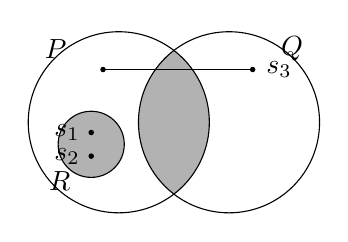
\begin{tikzpicture}[x=1cm,y=1cm]
\begin{scope} \clip (0,0) circle (1.15);
  \fill[black!30] (1.4,0) circle (1.15); \end{scope}
\fill[black!30] (-.35,-.28) circle (.42);
\draw (0,0) circle (1.15); \draw (1.4,0) circle (1.15);
\draw (-.35,-.28) circle (.42);
\node at (-.8,.93) {$P$}; \node at (2.2,.93) {$Q$};
\node at (-.75,-.75) {$R$};
\fill (-.35,-.13) circle (.035); \node[left] at (-.37,-.13) {$s_1$};
\fill (-.35,-.43) circle (.035); \node[left] at (-.37,-.43) {$s_2$};
\draw (-.2,.67)--(1.7,.67);
\fill (-.2,.67) circle (.035); \fill (1.7,.67) circle (.035);
\node[right] at (1.75,.67) {$s_3$};
\end{tikzpicture}
\caption{Native spider reconstruction of the chapter's exact-cardinality
example. The shaded overlap is empty because no spider inhabits it;
the shaded \(R\)-region has exactly its two distinct witnesses.}
\label{fig:p12-r131-spider-cardinality}
\end{figure}

\begin{hbtheorem}{thm:p12-r131-cardinality}{proved=annex:p12.r131.cardinality}{The spider example's exact reading}
The diagram in \cref{def:p12-r131-spider-cardinality}, interpreted by
\cref{def:p12-r131-spider-semantics}, is equivalent to the assertion
\[
\begin{gathered}
 R\subseteq P,\quad P\cap Q=\varnothing,\\
 \exists s_1,s_2,s_3\in U\;
 \bigl(s_1,s_2,s_3\text{ pairwise distinct}\ \land\
 R=\{s_1,s_2\}\ \land\ s_3\in(P\setminus R)\cup Q\bigr).
\end{gathered}
\]
The bound is on \(R\), not on all of \(P\), \(Q\), or \(U\).
\end{hbtheorem}

The source assigns Venn-II the expressive power of monadic first-order
logic without equality, and spider diagrams that of monadic first-order
logic with equality. Distinctness and upper bounds explain why spiders
can express exact cardinalities that a lone existential mark does not.
The 2005 spider calculus and Speedith's 2015 extension are not identical:
the latter explicitly adds implication, biconditional and negation to the
earlier conjunction/disjunction language and proves completeness for the
enlarged system. The full named-system metatheorems are cited results,
not consequences of the few example transformations below
\cite[pp.~718,722]{Jamnik2021LogicalDiagrams}
\cite[sec.~3.4, appendices~2--3]{UrbasJamnikStapleton2015Speedith}.

\section{The selected diagram rules and their direction}

\calculussheet{sheet:p12-r131-speedith-fragment}{Selected Speedith spider transformations}{Language: unitary tuples $d=(L,Z,\mathrm{ShZ},S,\eta)$ and classical compound diagrams; judgments: semantic consequence under the declared spider interpretation; negation: classical compound connective, not included in this rule fragment; equality: distinct spider witnesses in the semantics. This is the fragment needed by the worked example, not the complete Speedith calculus.}
\hbrule{rule:p12-r131-addfeet}{AddFeet}{d}{d[s:\eta(s)\cup h]}{$s\in S$; $h\subseteq Z\setminus\eta(s)$; all other fields unchanged; forward consequence only}
\hbrule{rule:p12-r131-splitspider}{SplitSpider}{d}{d[s:r]\lor d[s:\eta(s)\setminus r]}{$\varnothing\ne r\subsetneq\eta(s)$; all other fields unchanged; the rule is an equivalence and can also be used in reverse}
\hbrule{rule:p12-r131-removeshading}{RemoveShading}{(L,Z,\mathrm{ShZ},S,\eta)}{(L,Z,\mathrm{ShZ}\setminus r,S,\eta)}{$r\subseteq\mathrm{ShZ}$; forward consequence only}
\hbrule{rule:p12-r131-introshadedzone}{IntroduceShadedZone}{(L,Z,\mathrm{ShZ},S,\eta)}{(L,Z\cup\{z\},\mathrm{ShZ}\cup\{z\},S,\eta)}{$z$ is a missing Boolean zone for $L$; no new spider foot is added; the rule is an equivalence and can also be used in reverse}


The sheet records a fragment of the actual Speedith rules needed here,
not a claim to present its full complete calculus. In the notation
\(d[s:h]\), replace only spider \(s\)'s habitat by \(h\), leaving
all other tuple fields unchanged. Enlarging a habitat forgets location
information. Splitting a habitat gives alternative whole diagrams,
with a fresh existential spider map in each alternative. Neither is a
movement of a named physical individual from one set to another.

\begin{hbtheorem}{thm:p12-r131-rules}{proved=annex:p12.r131.rules}{Soundness of the displayed rule fragment}
AddFeet and RemoveShading preserve semantic consequence in the displayed
direction. SplitSpider and IntroduceShadedZone preserve the unitary
assertion in both directions. AddFeet is not generally reversible.
These claims use the tuple semantics, nonempty habitat side conditions
and classical compound connectives on the sheet.
\end{hbtheorem}

\section{Three implementations, three proof choices}

\subsection{Hyperproof: symbolic assertions and a partial block world}

Hyperproof combines first-order sentences with a graphical block-world
situation. In the source's figure~13.1.7 the given sentences include
\(\operatorname{Dodec}(c)\to\operatorname{Dodec}(d)\) and
\(\operatorname{Small}(c)\). Applying the situation and inspecting it
supplies \(\operatorname{Dodec}(c)\); implication elimination gives
\(\operatorname{Dodec}(d)\), and inspecting the resulting exhaustive
shape possibilities establishes \(\operatorname{SameShape}(c,d)\).
The smallness premise helps identify/constrain the situation; it is not
itself a shape theorem \cite[p.~719]{Jamnik2021LogicalDiagrams}.

\begin{hbtheorem}{thm:p12-r131-hyperproof}{proved=annex:p12.r131.hyperproof}{The observed-shape inference and its missing-premise contrast}
Suppose the situation licenses \(\operatorname{Dodec}(c)\), the
implication premise holds, and two dodecahedra count as the same shape
under the task's shape convention. Then
\(\operatorname{SameShape}(c,d)\) follows. The two given sentences
alone, without the observation, need not imply that conclusion.
\end{hbtheorem}

The source describes Kleene evaluation for partially specified situations:
every accepted symbolic or diagrammatic step must meet the declared
evaluation criterion. An unknown shape is not made known by an attractive
rendering. The displayed derivation is a fully justified classical
consequence under an explicit observation, not a verification of every
Hyperproof rule or software component. The diamond icon in the interface
denotes the situation and opens its graphic display; it is not another
geometric premise.

\subsection{Diamond: concrete dot arrays and uniform proofs}

Diamond works with natural-number arithmetic and diagrammatic proofs of
inductive claims. The source's concrete \(n=6\) square is partitioned
into nested L-shaped layers, or \emph{ells}. The two perpendicular
edges of an ell of size \(k\) contain \(k+k-1=2k-1\) dots,
because their corner would otherwise be counted twice. An \emph{lcut}
separates one ell from the remaining smaller square. The source performs
five cuts before reaching the one-dot base case
\cite[pp.~719--720, note~8]{Jamnik2021LogicalDiagrams}.

\begin{figure}[htbp]
\centering
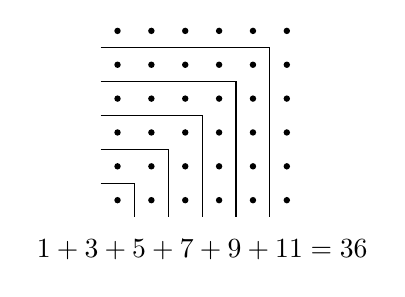
\begin{tikzpicture}[x=.43cm,y=.43cm]
\foreach \i in {1,...,6}{\foreach \j in {1,...,6}{
 \fill (\i,\j) circle (.095);}}
\foreach \k in {2,...,6}{\draw (0.5,\k-.5)--(\k-.5,\k-.5)--(\k-.5,.5);}
\node[align=center] at (3.5,-.45) {$1+3+5+7+9+11=36$};
\end{tikzpicture}
\caption{The six-by-six dot square partitioned into ells, independently
redrawn from the source's arithmetic example. The finite instance
motivates a recursive decomposition but does not by itself prove it
for every square size.}
\label{fig:p12-r131-ells}
\end{figure}

\begin{hbtheorem}{thm:p12-r131-odd-sum}{proved=annex:p12.r131.odd-sum}{Uniform correctness of the ell decomposition}
For each standard natural number \(n\geq0\), the finite dot square
\(D_n=\{1,\ldots,n\}^2\) is partitioned by the layers
\(L_k=D_k\setminus D_{k-1}\), \(1\leq k\leq n\), each with
\(2k-1\) elements. Recursive lcut down to the empty square is total,
preserves the dots without duplication, and produces this partition.
Consequently \(\sum_{k=1}^{n}(2k-1)=n^2\), with the empty sum zero.
Stopping at \(D_1\) instead leaves that one-dot base layer and takes
\(n-1\) cuts when \(n\geq1\).
\end{hbtheorem}

Jamnik invokes a constructive omega-rule to justify generality from a
uniform effective proof-producing procedure. The obligation is not
discharged by writing a recursive program or guessing a pattern from
two pictures. The Diamond primary explicitly separates conjectured
abstraction from verifying, in a metatheory, that the program supplies
appropriate diagram conversions and valid applicable operations for
\emph{every} input \cite[pp.~309--314]{JamnikBundyGreen1999Arithmetic}.
The annex supplies that verification for this lcut procedure. A uniform
family of standard-natural-number instances should not be confused with
a finitary first-order universal-introduction rule valid without further
assumptions in every nonstandard arithmetic model.

\subsection{Speedith: habitat weakening and explicit case splitting}

Speedith is an interactive prover for spider diagrams. Its source example
begins with two distinct witnesses: \(t_2\in A\cap B\) and
\(t_1\in(A\setminus B)\cup(B\setminus A)\). The target merely
requires distinct witnesses \(u_1\in A\) and \(u_2\in B\).
Names may be reselected when existential witnesses are assigned; the
target is not a demand that the same leftmost named spider remain in
the same set in every proof branch.

\begin{figure}[htbp]
\centering
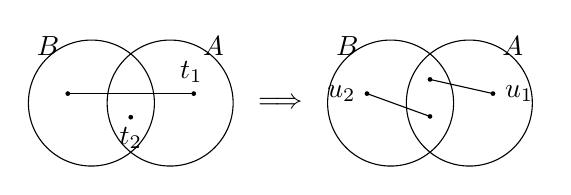
\begin{tikzpicture}[x=1cm,y=1cm]
\draw (0,0) circle (.8); \draw (1,0) circle (.8);
\node at (-.55,.72) {$B$}; \node at (1.55,.72) {$A$};
\draw (-.3,.12)--(1.3,.12);
\fill (-.3,.12) circle (.03); \fill (1.3,.12) circle (.03);
\node[above] at (1.27,.14) {$t_1$};
\fill (.5,-.18) circle (.03); \node[below] at (.5,-.18) {$t_2$};
\node at (2.4,0) {$\Longrightarrow$};
\begin{scope}[xshift=3.8cm]
\draw (0,0) circle (.8); \draw (1,0) circle (.8);
\node at (-.55,.72) {$B$}; \node at (1.55,.72) {$A$};
\draw (-.3,.12)--(.5,-.17);
\fill (-.3,.12) circle (.03); \fill (.5,-.17) circle (.03);
\node[left] at (-.32,.12) {$u_2$};
\draw (.5,.3)--(1.3,.12);
\fill (.5,.3) circle (.03); \fill (1.3,.12) circle (.03);
\node[right] at (1.33,.12) {$u_1$};
\end{scope}
\end{tikzpicture}
\caption{Initial and final assertions of the source's Speedith proof,
redrawn as native spiders. Each connecting line denotes alternative
locations of one witness, not a path an element travels.}
\label{fig:p12-r131-speedith}
\end{figure}

The complete transformation in the chapter's figure~13.1.9 is as follows.
SplitSpider first separates the two possible habitats of \(t_1\),
producing a disjunction of two diagrams. In the branch where
\(t_1\in A\setminus B\), two AddFeet operations enlarge \(t_1\)'s
habitat to \(A\) and \(t_2\)'s to \(B\). In the other branch,
two AddFeet operations enlarge \(t_1\)'s habitat to \(B\) and
\(t_2\)'s to \(A\). Renaming witness handles makes the two weakened
diagrams identical; idempotency collapses their disjunction, and the
remaining implication of a diagram by itself is a tautology.
These are six substantive transformations: one split, four habitat
enlargements and one idempotency step, followed by closing the implication
\cite[pp.~720--721]{Jamnik2021LogicalDiagrams}
\cite[p.~489, fig.~1]{UrbasJamnikStapleton2015Speedith}.

\begin{hbtheorem}{thm:p12-r131-speedith}{proved=annex:p12.r131.speedith}{Validity and loss of information in the Speedith example}
The initial spider assertion in \cref{fig:p12-r131-speedith} entails
the final assertion. The converse fails: two distinct witnesses, one
in \(A\) and one in \(B\), need not include a witness in
\(A\cap B\).
\end{hbtheorem}

The three systems therefore address different interfaces. Hyperproof
mixes a situation with sentences; Diamond checks a recursive family
of concrete arithmetic derivations; Speedith applies rules to abstract
unitary/compound spider syntax and displays the results. Soundness is
necessary for accepting their proofs; completeness is a separate
coverage property. Layout quality, abstraction level, user interaction
and proof readability remain design decisions even when both properties
hold. The Speedith primary separates abstract representation, reasoning
kernel, external communication and graphical layout. A diagram can be
logically correct yet badly drawn; a correctly executed drawing algorithm
does not itself prove the logical rules sound. These distinctions connect
to \cref{def:p12-mechanization-layers,def:p12-deep-shallow-embedding}.

\section{Expressive, cognitive and evidential limits}

The source also mentions Grover for analogical mathematical reasoning,
iCon for ontologies, and UML specifications based on higraphs. These are
examples of distinct formalization projects, not interchangeable complete
proof systems. Likewise, a formal four-color proof illustrates the reach
of sentential proof assistants, not a theorem that diagrams are never
useful \cite[pp.~718,722]{Jamnik2021LogicalDiagrams}.
Spider diagrams' monadic fragment does not supply arbitrary binary
relations, and Diamond's stated shape-based arithmetic domain does not
cover every arithmetic theorem. Intended concreteness must be separated
from incidental visual features: the example size six is intended for
display but not a premise restricting the universal theorem; arbitrary
curve areas and spacing have no meaning in the set semantics.

Jamnik proposes accessibility and explanation as reasons to investigate
diagrammatic reasoning, drawing on mental-model, clutter and individual-
difference literature. These are not theorems of the diagram calculus.
The cited machine-comprehension work by Hegarty and Just concerns text
and diagrams of machines; the Alqadah study concerns Euler interpretation
and clutter; Stenning and Oberlander distinguish logical equivalence from
processing properties and discuss external graphics and internal reasoning.
Those tasks are not the checkerboard, general theorem proving or mental
rotation. The chapter supplies no study samples, assignments, quantitative
estimates or uncertainty intervals sufficient to infer an all-user benefit.
Its report of successful Hyperproof classroom deployment similarly does
not specify a controlled comparison or a measured general effect.
Accordingly, these remain attributed motivations with unresolved
study-level qualification, not prescriptions established by empirical data
\cite[pp.~717,719,722, note~7]{Jamnik2021LogicalDiagrams}.
The evidence discipline is that of \cref{def:p19-evidence-record}:
population, task, design, measures, uncertainty, alternative explanation
and replication/generalization must be supplied before such claims are
used as empirical conclusions. An external display's usefulness would
not uniquely identify an internal cognitive mechanism in any case.

For consultation, choose a diagram by the information the task actually
needs. Preserve the stated premises and all alternatives; declare what
missing zones, marks, shading and names mean; use a sound transformation
with its side conditions; and check whether the conclusion is genuinely
general or only about the displayed instance. The checkerboard, free
ride, shaded-cardinality and Speedith examples supply successful cases.
Reversing AddFeet, inferring existence from drawn area, reading the
unasserted relation of one possible model, or generalizing from one
dot square supply concrete failure cases. Representation selection
remains a research and engineering problem, rather than a guarantee
that every problem or every person benefits from pictures.
